\documentclass[dvipsnames] {beamer}
\usepackage{cmlgc}
\usepackage{comment}
\usepackage{tikz}
\usefonttheme{serif}     % Font theme: serif
\usepackage[T2A]{fontenc}
\usepackage[utf8]{inputenc}
\usepackage[english]{babel}
\usepackage{amssymb,amsfonts,amsmath,mathtext,cite,enumerate,float} %подключаем нужные пакеты расширений
% \usepackage{cyrillic}
\usepackage{color, colortbl}
\usepackage{multirow}
\usepackage{graphicx}
\usepackage{graphics}
\usepackage{multirow}
\usepackage{url}
\usepackage{hyperref}
\usepackage{animate}
\usepackage{pifont}
\usepackage{wasysym}
\usepackage{marvosym}
\usepackage{appendixnumberbeamer} 
\usepackage{pgfpages}
\usepackage{systeme,mathtools}
\usepackage{mathtools}
\usepackage{listings}
\usepackage{xcolor} % for setting colors
\usepackage{mhchem}


\usepackage{ragged2e} %выравнивание текста по ширине слайда (\justifying)
%\setbeamercolor{background canvas}{bg=violet}

\usetheme{Madrid}
%\usecolortheme{crane}

%=================================================

\defbeamertemplate*{footline}{mytheme}{%
  \leavevmode%
  \hbox{%
    \begin{beamercolorbox}[wd=.2\paperwidth,ht=3ex,dp=1ex,center]{author in head/foot}%
      \usebeamerfont{author in head/foot}\insertshortauthor
    \end{beamercolorbox}%
    \begin{beamercolorbox}[wd=.7\paperwidth,ht=3ex,dp=1ex,center]{title in head/foot}%
      \usebeamerfont{title in head/foot}\insertshorttitle
    \end{beamercolorbox}%
    \begin{beamercolorbox}[wd=.1\paperwidth,ht=3ex,dp=1ex,right]{date in head/foot}%
      %\usebeamerfont{date in head/foot}\insertshortdate{}\hspace*{2em}
      %\insertframenumber{} / \inserttotalframenumber\hspace*{2ex} %номер текущего слайда / общее число слайдов
      \insertframenumber{} \hspace*{5ex}  %номер текущего слайда
  \end{beamercolorbox}}%
  \vskip0pt%
}
\usebeamertemplate{mytheme}
\beamertemplatenavigationsymbolsempty

\defbeamertemplate*{frametitle}{boldTitle}{%
  \begin{beamercolorbox}[wd=\paperwidth,ht=3ex,dp=3pt,center]{title in head/foot}%
    %        \ \textit{\textbf{\insertframetitle}} % курсивный заголовок слайда 
    \ \textbf{\insertframetitle}
  \end{beamercolorbox}
}
\usebeamertemplate{boldTitle}
\setbeamercovered{dynamic}

\setbeameroption{hide notes} % Only slides
%\setbeameroption{show only notes} % Only notes
%\setbeameroption{show notes on second screen=right} % Both
%\setbeamertemplate{note page}[plain]


%=================================================
% \titlegraphic{\includegraphics[width=\textwidth]{logo_conf.png}}

\addtobeamertemplate{title page}{\centering \includegraphics[scale=0.3]{jinr_nica_logo_spbuAdded.png}}{}
\addtobeamertemplate{title page}{\centering \includegraphics[scale=0.45]{dubna.png}}{}
%\addtobeamertemplate{title page}{\centering \includegraphics[scale=0.095]{wpcf2018_2.png}}{}

\title[\bf Семинар «Ускорительный комплекс NICA — проект мега-класса»]{\textbf{\large {Эксперименты BM@N и MPD на ускорительном комплексе NICA}}}

\author[\bf П. Батюк]{\textbf{{\footnotesize П. Батюк, pavel.batyuk@jinr.ru}}} 
\institute{\bf Лаборатория физики высоких энергий им. Векслера и Балдина (ЛФВЭ), \\ Объединённый институт ядерных исследований, Дубна}
\date{}
% \newpage \footnotesize April 14, 2016}}

\lstset{
  %    frame=tb, % draw a frame at the top and bottom of the code block
  tabsize=4, % tab space width
  showstringspaces=false, % don't mark spaces in strings
  %   numbers=left, % display line numbers on the left
  commentstyle=\color{blue}, % comment color
  keywordstyle=\color{blue}, % keyword color
  stringstyle=\color{red} % string color
}

\graphicspath{{../common_figures/}}

\begin{document}
\maketitle



\begin{frame}
  \bf
  \frametitle{Ускорительный комплекс NICA}
  \vskip -.8cm
  \begin{columns}[t]
    \column{.49\textwidth}
            {\footnotesize
    \begin{block}{}
      \begin{figure}[H]
        \includegraphics[width=1.\linewidth]{nica_complex1.png}
      \end{figure}
      %\centering The general contractor is  {\color{red} STRABAG} (Bodostal-3 \& PCJ are the sub-contractors)
    %\end{block}
    \vskip -.8cm

   % \begin{block}{}
      \begin{itemize}
      \item Набор ускорителей для обеспечения пучков частиц, которые будут использованы в экспериментах
      \item Экспериментальные установки
      \item Линии для сборки и проверки сверхпроводящих магнитов
      \item Помещения для проектирования и сборки детекторов
      \item Инновационный центр
      \end{itemize}
    \end{block}
        }
            \column{.49\textwidth}
            {\footnotesize 
              \begin{block}{}
                \vskip -.2cm
      \centering  Пучки - {\color{red}$p$, $d$ ... $^{197}Au^{79+}$} \\
      \centering  Энергия столкновения: \\
        $\sqrt{s_{NN}}$ = {\color{red} 4 - 11} ГэВ
        $E_{lab}$ =  {\color{red}1 - 6} ГэВ/н \\
      Светимость: {\color{red}$10^{27}~cm^{-2}s^{-1}$}(Au), {\color{red}$10^{32}$}(p) \\
 \end{block}
 \vskip -.4cm
 \begin{block}{}
      \begin{itemize}
      \item 2 точки встречи пучков - {\color{red}MPD} и {\color{red}SPD}
      \item Эксперимент в режиме фиксированной мишени -  {\color{red}BM@N}
      \end{itemize}
 \end{block}
 \vskip -.4cm
 \begin{block}{}
      \begin{itemize}
      \item {\color{red} 2018:} Выведенные пучки аргона и криптона были доступны в эксперименте BM@N
      \item {\color{red} 2020-2021}: Эксперимент MPD в стартовой конфигурации.
      \item {\color{red} 2023}: Полностью готовый комплекс NICA согласно проектному заданию.	
      \end{itemize}
 \end{block}
 }
  \end{columns}
\end{frame}

\begin{frame}
  \frametitle{\bf \centering Нуклотрон (в работе с 1993)}
  \vskip -.75cm
  \begin{columns}[t]
    \column{.49\textwidth}
    \begin{block}{\bf \centering Модернизирован в 2010 - 2015}
      \bf 
      \resizebox{\columnwidth}{!}{%
        \begin{tabular}{| l | l |}
          \hline			
          Параметры & Нуклотрон \\
          \hline
          Тип & Сверхпроводящий синхротрон \\
          \hline 
          Частицы & $\uparrow$p, $\uparrow$d, тяжёлые ядра \\
          \hline
          Макс. кин. энергия [ГэВ/н] & 12.07 ($\uparrow$p), 5.62 ($\uparrow$d), 4.38 (Au) \\
          \hline
          Магнитная жёсткость [T $\cdot$ m] & 25 - 43.25 \\
          \hline
          Периметр [m] & 251.52 \\
          \hline
          Вакуум [Торр] & $10^{-9}$ \\
          \hline
          Интенсивность, Au [ионов/сброс] & 1 $\cdot 10^{9}$ \\
          \hline
          % transition energy [GeV/u] & 7.0 \\
          %  \hline
          Время медленного вывода [с] & вплоть до 10 \\
          \hline
        \end{tabular}
      }
    \end{block}
     \vskip -.3cm
    {\bf
    \begin{block}{}
      \begin{itemize}
      \item Проект ускорителя был одобрен в {\color{red} 1986}
      \item Сборка \& первые пучки, {\color{red} Март 1993}
      \item Медленный вывод {\color{red} 2000}
      \end{itemize}
     % \vskip .6cm
      \begin{center}
        Тяжёлые ионы  от p до Xe \\
        (C, Mg, Fe, Ar, Kr) \\
        Поляризованные протоны и дейтроны
      \end{center}
    \end{block}
    }
    
    \column{.49\textwidth}
    \begin{block}{}
      \begin{figure}[H]
        \includegraphics[width=1.\linewidth]{nuclotron1.png} \\
        \includegraphics[width=1.\linewidth]{nuclotron2.png}
      \end{figure}
    \end{block}
  \end{columns}
\end{frame}


\begin{frame}
  \frametitle{\bf \centering Нуклотрон, сеансы для физиков}
   \vskip -.75cm
  \begin{columns}[t]
    \column{.47\textwidth}
    \begin{block}{\bf \centering \footnotesize Сеанс № 53, 1450 часов, один из самых продолжительных}
      \begin{figure}[H]
        \includegraphics[width=1.\linewidth]{run53.png}
      \end{figure}
    \end{block}
    \vskip -0.2cm
    {\footnotesize 
    \begin{block}{}
      \begin{itemize}
      \item {\bf {\color{red} Сеанс 53} - Поляризованные и неполяризованные дейтроны, макс. кин. энергия -  4.6 ГэВ/н}
      \item {\bf {\color{red} Сеанс 54} - Пучок ионов углерода}
      \item {\bf {\color{red} Сеанс 55} - Пучки ионов аргона и криптона}
      \end{itemize}
    \end{block}
    }
    \column{.47\textwidth}
     \begin{block}{\bf \centering \footnotesize Сеанс № 54, 1150 часов}
       \begin{figure}[H]
         \includegraphics[width=1.\linewidth]{run54.png}
       \end{figure}
     \end{block}
      \begin{block}{\bf \centering \footnotesize Сеанс № 55: Февраль - Апрель, 2018}
      \begin{figure}[H]
        \includegraphics[width=1.\linewidth]{run55.png} \\
      \end{figure}
    \end{block}    
  \end{columns}  
\end{frame}

\begin{frame}
  \frametitle{\bf \centering Бустер}
  \vskip -.75cm
  \begin{columns}[t]
    \column{.6\textwidth}
    \begin{block}{\bf \centering {\small Сборка была начата в 2018}}
      \bf
      \resizebox{\columnwidth}{!}{%
        \begin{tabular}{| c | c |}
          \hline	
          Параметры & Бустер \\
          \hline
          Тип & Сверхпроводящий синхротрон \\
          \hline
          Частицы & ионы с $A/Z \leq 3$ \\
          \hline
          Энергия вброса [MeV/u] & 3.2 \\
          \hline
          Энергия вывода [MeV/u] & 600 \\
          \hline
          Магнитная жёсткость [T $\cdot$ м] & 1.6 - 25.0 \\
          \hline
          Периметр [м] & 210.96 \\
          \hline
          Вакуум [Торр] & $10^{-11}$ \\
          \hline
          Интенсивность [Au ионов/сброс] & $1.5 \cdot 10^{9}$ \\
          \hline
        \end{tabular}
      }
      %\vskip -.3cm
      \begin{figure}[H]
        \includegraphics[width=1.\linewidth]{booster_tunnel2_2019.jpg} 
      \end{figure}
    \end{block}
    %\begin{block}{\bf \centering {\small RF stations are tested}}
    %\begin{figure}[H]
    %  \includegraphics[width=1.\linewidth]{booster3.png} 
    %\end{figure}
    %\end{block}

    \column{.35\textwidth}
    \begin{block}{\bf \centering {\small Туннель для бустера}}
      \begin{figure}[H]
        \includegraphics[width=1.\linewidth]{booster_tunnel_2019.jpg} 
      \end{figure}
    \end{block}
    \vskip -.3cm
    %\begin{block}{\bf \centering {\small Electron Cooling System}}
    %  \begin{figure}[H]
    %    \includegraphics[width=1.\linewidth]{booster2.png}
    %  \end{figure}
    %\end{block}
    {\scriptsize \bf 
    \begin{block}{}
      \begin{itemize}
        \item  Сборка магнитной системы закончена.
        \item  Начало сборки - Сентябрь 2018.
        \item Первый (технологический) сеанс - весна 2020.
        \item Полное соответствие проекту - конец 2020, начало 2021 года        
      \end{itemize}
      {\color{red} Первый магнит был установлен 19 сентября 2018}
    \end{block}
    }
  \end{columns}
\end{frame}



\begin{frame}
  \bf
  \frametitle{\bf \centering \footnotesize Линия для сборки и проверки сверхпроводящих магнитов}
  \vskip -.75cm
  \begin{columns}[t]
    \column{.48\textwidth}
    \begin{block}{\bf \centering Основные элементы (зоны):}
      %\vskip -.15cm
      \begin{itemize}
      \item Проверка сверхпроводящих кабелей и обмоток
      \item Сборка магнитов
      \item "Тёплые'' магнитные измерения
      \item Проверка на предмет утечек
      \item "Холодные'' магнитные измерения
      \end{itemize}   
    \end{block}
    \vskip -0.35cm
    \begin{block}{}
      {\color{red} Все магниты для Бустера сделаны и проверены в Дубне!}
    \end{block}
    
    \column{.39\textwidth}
    \begin{block}{}
      \begin{figure}[H]
        \includegraphics[width=1.\linewidth]{SC_magnetLine.png} \\
        \includegraphics[width=1.\linewidth]{SC_assemblingHall.png}
      \end{figure}
    \end{block}
    \vskip -.3cm
    \begin{block}{}
      {\footnotesize \color{red} \bf \centering 450 магнитов для ускорительных комплексов NICA и FAIR}
    \end{block}
  \end{columns}
\end{frame}

\begin{frame}
  \frametitle{\bf \centering Источник тяжёлых ионов KRION 6T}
  \begin{columns}[c]
    \column{.125\textwidth}   
    \column{.75\textwidth}
    \begin{block}{\bf \centering Был использован в сеансе №55}
      \begin{figure}[H]
        \includegraphics[width=1.\linewidth]{krion6T.jpg} 
      \end{figure}
    \end{block}
    \column{.125\textwidth}
      \end{columns}
    {\bf 
    \begin{block}{}
      \begin{itemize}
      \item Способен обеспечивать порядка $2.5 \cdot 10^{9}$ ионов золота $Au^{31+}$ за цикл. Частота цикла - 10 Гц.
      \end{itemize}
    \end{block}
    } 
\end{frame}

\begin{frame}
  \frametitle{\bf \centering Линейные ускорители}
  \vskip -.75cm
  \begin{columns}[t]
    \column{.44\textwidth}
    \begin{block}{\bf \centering ЛУ-20}
      \begin{figure}[H]
        \includegraphics[width=1.\linewidth]{lu20.jpg} 
      \end{figure}
    \end{block}
    
    \column{.52\textwidth}
    \begin{block}{\bf \centering HILAC}
      \begin{figure}[H]
        \includegraphics[width=1.\linewidth]{hilac.jpg} 
      \end{figure}
    \end{block}
       
  \end{columns}
   {\bf \footnotesize 
     \begin{block}{}
       \begin{center}
            \begin{itemize}
            \item {\color{red} ЛУ-20} - ОИЯИ (Дубна), ИЯИ (Троицк), ИТЭФ (Москва), МИФИ (Москва) (Сборка - {\color{blue} Май 2016})
            \item {\color{red} HILAC} - BEVATECH OHG (Сборка - {\color{blue} Октябрь 2018})
            \end{itemize}
       \end{center}
          \end{block}
   }
   \vskip -0.3cm
    \begin{block}{}
       \bf
      \resizebox{\columnwidth}{!}{%
        \begin{tabular}{| c | c | c |}
          \hline	
           & ЛУ-20 & HILAC \\
          \hline
          Отношение $A / Z$ & 1-3 & 1-6 \\
          \hline
          Энергия вброса [КэВ / а.е.м.] & 150 for A/Z 1-3 & 17 \\
          \hline
          Энергия вывода [МэВ / а.е.м.] & 5 (A/Z 1-3) & 3.24 (A/Z = 6) \\
          \hline
        \end{tabular}
      }
    \end{block}
\end{frame}

\begin{frame}
  \frametitle{\bf \centering Коллайдер}
  \vskip -0.75cm
  \begin{columns}[t]
    \column{.15\textwidth}
    
    \column{.7\textwidth}
     \begin{block}{\bf \centering Официальное начало строительства {\color{red} 25 Марта 2016}}
      \begin{figure}[H]
        \includegraphics[width=1.\linewidth]{collider_start.jpg} 
      \end{figure}
     \end{block}

     \column{.15\textwidth}
     
  \end{columns}
\end{frame}

\begin{frame}
  \bf
  \frametitle{\bf \centering Коллайдер}
  \vskip -.25cm
  \begin{block}{}
     \centering \url{http://nucloweb.jinr.ru/nucloserv/205corp.htm}
  \end{block}
  \vskip -.66cm
  \begin{columns}[t]
    \column{.49\textwidth}
   % \begin{block}{\bf \centering NICA site online \\ \url{http://nucloweb.jinr.ru/nucloserv/205corp.htm}}
    \begin{block}{}
    \begin{figure}[H]
        \includegraphics[width=1.\linewidth]{collider_online.png} \\
        \includegraphics[width=1.\linewidth]{Screenshot_20190909_101022.png}
      \end{figure}
    \end{block}
    %\begin{block}{}

    %\end{block}
    \column{.49\textwidth}
    \begin{block}{}
      \includegraphics[width=1.\linewidth]{NICA_collider_panPhoto.png}
    \end{block}
    \vskip -.3cm
    \begin{block}{\bf \centering Основные характеристики:}
      \resizebox{\columnwidth}{!}{%
        \begin{tabular}{| c | c |}
          \hline
          Периметр [м] & {\color{Red} 503.04} \\
          \hline
          Макс. энергия $\sqrt{s_{NN}}$ [ГэВ] & {\color{Red} 11} \\
          \hline
          $\Delta p / p$ $[10^{-3}]$ & 1.6 \\
          \hline
          Светимость [$cm^{-2} \cdot s^{-1}$] & {\color {Red} $10^{27}$} \\
          \hline
        \end{tabular}
        }

    \end{block}
  \end{columns}
\end{frame}

\begin{frame}
  \frametitle{\bf \centering Коллайдер}
  \begin{block}{\bf \centering Сентябрь 2018}
     \begin{figure}[H]
        \includegraphics[width=.8\linewidth]{collider_now.png} 
      \end{figure}
  \end{block}
\end{frame}

\begin{frame}
  \frametitle{\bf \centering Коллайдер}
  \begin{block}{\bf \centering Aвгуст 2019}
     \begin{figure}[H]
        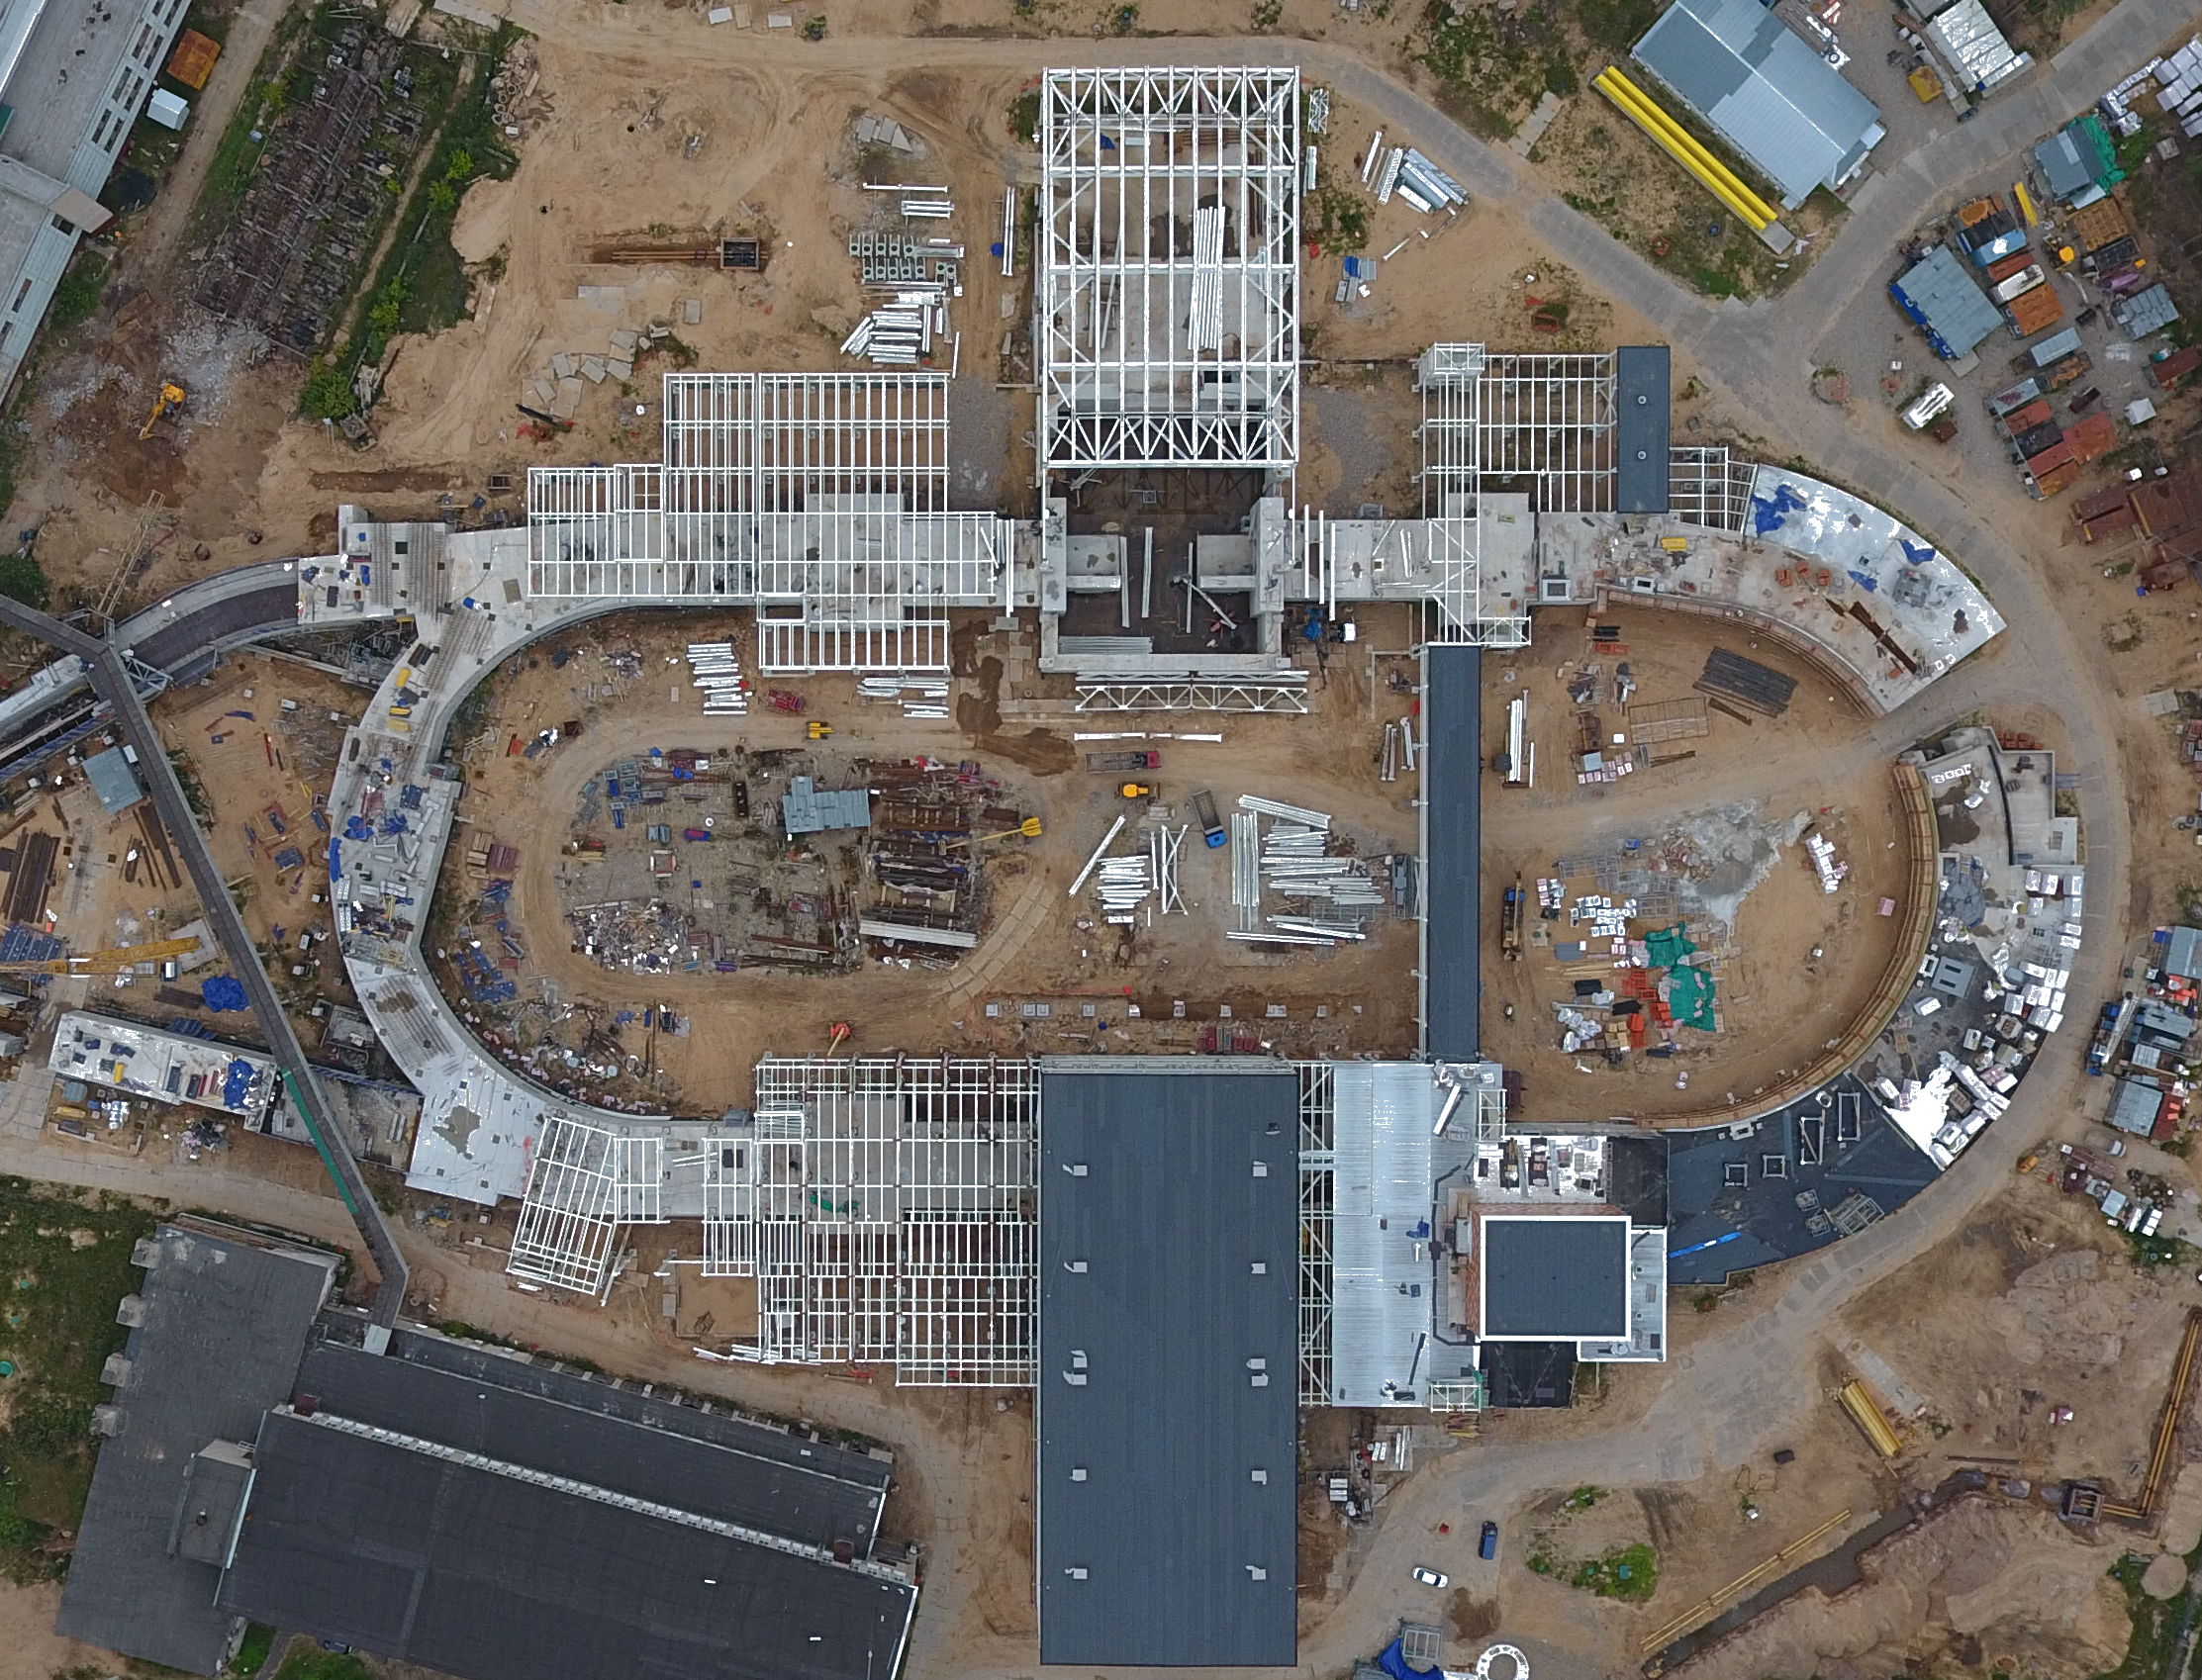
\includegraphics[width=.8\linewidth]{collider_August2019.png} 
      \end{figure}
  \end{block}
\end{frame}



\begin{frame}
  \bf
  \frametitle{\bf \centering \footnotesize Фазовая диаграмма состояния кварк-глюонной материи}
  \vskip -.75cm
  \begin{columns}[t]
    \column{.45\textwidth}
    \begin{block}{}
      \begin{figure}[H]
        \includegraphics[width=1.\linewidth]{qcd_diagram.png}
      \end{figure}
    \end{block}
    \vskip -.75cm

    \begin{columns}[t]
      \column{.48\textwidth}  
      \begin{block}{\bf \centering {\tiny Высокие энергии:}}
        {\tiny
          \begin{itemize}
          \item Количество барионов и антибарионов совпадает
          \item КХД предсказывает быстрый и гладкий переход между адронной и партонной материей
         % \item ALICE, ATLAS, CMS, STAR, PHENIX
          \end{itemize}
        }
      \end{block}
      \column{.48\textwidth}
      \begin{block}{\bf \centering {\tiny Низкие энергии:}}
        {\tiny
          \begin{itemize}
          \item Барионы доминируют
          \item {\color {red} Фазовый переход первого рода? Экзотические состояния?}
          \item BES @ RHIC, NA61, CBM, {\color{red} NICA/MPD, BM@N}
          \end{itemize}
        }
      \end{block}
    \end{columns}

    \column{.51\textwidth}
    \begin{block}{\bf \centering \footnotesize Эксперименты, изучающие фазовую диаграмму}
      \vskip .25cm
      \begin{figure}[H]
        \includegraphics[width=1.\linewidth]{QCD_dense_matter_experiments.png}
      \end{figure}
    \end{block}
  \end{columns}
  \note{One of the most urgent task for the study of the QCD phase diagram is density frontier.
    According to various calculations maximum freeze-out density is reached at the energy range around $\sqrt{s_{NN}}$ = 10 GeV/n.
    So, NICA is well suited for exploring the transition between the hadronic and quark-gluon phases at the high net-baryon
    density. This is the top priority of the NICA program. \\
    The landscape of HIC experiments, present and future, in the energy
    region of max baryonic density are presented in this figure. Among fixed target experiments
    CBM at FAIR will provide maximum interaction rate. There are only two collider experiments – NICA and STAR BES with
    a difference in interaction rate of 3-4 orders of magnitude. Two NICA experiments - BM@N with fixed target and MPD
    at the collider will cover the whole indicated energy region.
  }
\end{frame}

\begin{frame}
  \bf
  \frametitle{\bf \centering Немного о физике, которую мы изучаем ...}
             {\footnotesize
               \vskip -.7cm
               \begin{columns}[t]
                 \column{.49\textwidth}
                 \begin{block}{\bf \centering Фазовая диаграмма}
                   \begin{figure}[H]
                     \includegraphics[width=1.\textwidth]{qcd_diagram.png} 
                   \end{figure}
                 \end{block}
                 \vskip -0.3cm
                 \begin{block}{\bf \centering Деконфайнмент при больших барионных плотностях}
                   % \vskip .25cm
                   \centering 
                       {\color{ForestGreen} увеличенный выход странных частиц} (одна из физ. задач эксперимента  BM@N) \\
                      % {\color{ForestGreen} Chiral Magnetic (vortical) effect, $\Lambda$-polarization}
                 \end{block}

                 \column{.49\textwidth}
                 \begin{block}{\bf \centering \footnotesize Уравнение состояния ядерной материи}
                   \centering
                       {\color{ForestGreen} выходы и спектры идентифицированных, частиц фемтоскопия, потоки} \\
                       {\color {Red} Измерения: $\gamma$, $\pi$, $K$, $p$, $\Lambda$, $\Omega$, античастицы, лёгкие ядра}
                 \end{block}
                 \vskip -0.3cm
                 \begin{block}{\bf \centering \footnotesize Модификации адронов в ядерной среде}
                   \centering 
                       {\color{ForestGreen} повышенный выход дилептонов с малыми массами} \\
                       {\color{Red} Измерения: $\rho$, $\omega$, $\phi$, $e^{+}e^{-}$}
                 \end{block}
                 \vskip -0.3cm
                 \begin{block}{\bf \centering \footnotesize Возможная критическая точка}
                   \centering 
                       {\color{ForestGreen} Пособытийные флуктуации (множественности)}
                 \end{block}
                 \vskip -0.3cm
                 \begin{block}{\bf \centering \footnotesize Странность в ядерной материи}
                   \centering 
                       {\color{ForestGreen} Гиперядра}
                 \end{block}
               \end{columns}
             }
\end{frame}

\begin{frame}
  \frametitle{\bf \centering Экспериментальная установка BM@N}
  \bf
       \vskip -.8cm
       \begin{columns}[t]
         \column{.69\textwidth}
         \begin{block}{}
           \begin{figure}[H]
             \includegraphics[width=1.\linewidth]{bmn_fullConfig.png}
           \end{figure}
         \end{block}

         \column{.29\textwidth}
         {\tiny
           \begin{block}{}
             \begin{itemize}
             \item Внутренний трекер внутри магнита для восстановления ядро-ядерных взаимодействий
             \item Внешний трекер за пределами магнитного поля 
             \item Времяпролётные детекторы для идентификации адронов и лёгких ядер
             \item Триггерные детекторы и пучковые мониторы
             \item Калориметры для измерения центральности взаимодействия и восстановления нейтральных частиц            
             \end{itemize}
           \end{block}
         }
       \end{columns}
       \vskip -.2cm
       {\footnotesize
         \begin{block}{\bf \centering {\scriptsize  Преимущества BM@N:}}
           \vskip -.1cm
         \begin{itemize}
         \item \centering Широкоапертурный анализирующий магнит
         \item Детекторные подсистемы устойчивы к большим множественностям заряженных частиц
         \item Идентификация частиц с помощью времяпролётной системы с широким покрытием фазового пространства
         \end{itemize}
       \end{block}
       }
\end{frame}

\begin{frame}
  \bf
  \frametitle{\bf \centering {\footnotesize Исследование плотной барионной материи на Нуклотроне}}
  \vskip -.75cm
  \begin{columns}[t]
    \column{.51\textwidth}
    \begin{block}{}
      \includegraphics[width=1.\linewidth]{bar_densities.png}
    \end{block}
    \column{.47\textwidth}
       \begin{block}{}
         \includegraphics[width=1.\linewidth]{barDensDomination.png}
       \end{block}
\end{columns}
  \begin{block}{}
    \begin{center}
  Нуклотрон позволяет получить плотную барионную материю, имеющую сравнительно большое время жизни.
    \end{center}
  \end{block}
\end{frame}

\begin{frame}
  \bf
  \frametitle{\centering Физика на Нуклотроне}
  % {\small
  \vskip -.75cm
               \begin{columns}[t]
                 \column{.49\textwidth} 
                 \begin{block}{\bf \centering $A+A$-взаимодействия:}
                   \begin{itemize}
                   \item Выход странных частиц
                   \item Более точные данные для странных мезонов, гиперонов, гиперядер
                   \end{itemize}
                 \end{block}
                 \begin{block}{\bf \centering $p+p$, $p+n$, $p+A$-взаимодействия :}
                   \begin{itemize}
                   \item Возможность изучить более детально эффекты ядерной среды
                   \end{itemize}
                 \end{block}
                 
                 \column{.44\textwidth} 
                 \begin{block}{\centering \bf {\color{yellow}{AGS}} {\color{red}{NA49}} {\color{ForestGreen}{BRAHMS}}}
                   %  \includegraphics[width=.4\linewidth]{strangeness_prod.png}
                   \includegraphics[width=1.\linewidth]{strangeness_prod.png}
                 \end{block}
                 %\begin{block}{}
                  % \includegraphics[width=1.\linewidth]{horn_NA49.png}
                 %\end{block}
               \end{columns}
               %  }
               \note{Production of strange particles in A+A collisions is of particular interest because their
                 enhanced yields (relative to pp reactions) have been predicted as the signal of the deconfinement phase
                 transition. Such enhancement, indeed, was observed at SPS energies and then confirmed at the RHIC.
                 However, the data on strangeness production, especially at threshold, at energy region of the maximum baryonic
                 density are not complete or even missing}
\end{frame}

\begin{frame}
  \bf
  \frametitle{\bf \centering BM@N, сеансы №53 (дейтроны) и 54 (углерод)}
  \vskip -.1cm
  \begin{block}{}
    \includegraphics[width=1.\linewidth]{bmn_winter2016_config_common_view_labels.png}
  \end{block}
  \vskip -.7cm
\end{frame}

\begin{frame}
  \vskip -.8cm
  \frametitle{\bf \centering  {$\Lambda^{0}$ в сеансах на дейтронах и углероде}}
  \begin{columns}[t]
    \column{.35\textwidth}
    {\footnotesize 
     \begin{block}{}
       \bf
       \begin{center}
       d (C) + мишень $\rightarrow$ X \\
       $\Lambda^{0}$-сигнал с шириной $\sim$ 2.5-3 МэВ
       \end{center}
     \end{block}
    % \vskip -.3cm
    % \begin{block}{}
    %   \begin{center}
    %     {\color{red} \bf No detailed PID used}
    %   \end{center}
    % \end{block}
     }
    % \vskip -.3cm
     \begin{block}{\bf \centering {\footnotesize Дейтроны}}
       \begin{figure}[H]
         \includegraphics[width=1.\linewidth]{lambda_run5.png} 
       \end{figure}
     \end{block}
    \column{.60\textwidth}
    \begin{block}{\bf \centering {\footnotesize Углерод}}  
      \begin{minipage}{.49\linewidth}
        \includegraphics[width=1.\linewidth]{lambda_all.png} \\ 
        \includegraphics[width=1.\linewidth]{lambda_Cu.png}
      \end{minipage}
      \begin{minipage}{.49\linewidth}
        \includegraphics[width=1.\linewidth]{lambda_C.png} \\
        \includegraphics[width=1.\linewidth]{lambda_Al.png}
      \end{minipage}
    \end{block}
  \end{columns}
\end{frame}

\begin{frame}
  \frametitle{\bf \centering \footnotesize Времяпролётные измерения в сеансе на углероде}
  \vskip -0.7cm
  \begin{columns}[t]
    \column{.44\textwidth}
   % \vskip -.82cm
    \begin{block}{\bf \centering {\scriptsize T = 3.5 ГэВ/н, C + Al $\rightarrow$ X}}
     % \vskip -.35cm
      \begin{figure}[H]
        \includegraphics[width=1.\linewidth]{tof400_res.png}
      \end{figure}
      \vskip -.75cm
      \begin{figure}[H]
        \includegraphics[width=1.\linewidth]{tof400_pid.png}
      \end{figure}
    \end{block}
    
    \column{.44\textwidth}
    %\vskip -.82cm
    \begin{block}{\bf \centering {\scriptsize T = 4.5 ГэВ/н, C + Cu $\rightarrow$ X}}
      %\vskip -.35cm
      \begin{figure}[H]
        \includegraphics[width=1.\linewidth]{tof700_res.png}
      \end{figure}
      \vskip -.75cm
      \begin{figure}[H]
        \includegraphics[width=1.\linewidth]{TOF700_PID.png}
      \end{figure}
    \end{block}
  \end{columns}
\end{frame}


\begin{frame}
  \bf
  \frametitle{\bf \centering BM@N,сеанс №55 (аргон и криптон)}
  \vskip -.9cm
  \begin{block}{}
     \begin{center}
       \includegraphics[width=1.\linewidth]{BMN_setup_RunSpring2018_back_labels.png}
     \end{center}
   \end{block}
\end{frame}

\begin{frame}
  \bf
  \frametitle{\bf \centering BM@N, сеанс №55, детекторные подсистемы}
  \vskip -.1cm
  \begin{columns}[t]
    \column{.51\textwidth}
    %\begin{figure}[H]
      \includegraphics[width=1.\linewidth]{GEMs.png} \\
    %\end{figure}
    %\begin{minipage}{.49\linewidth}
  % \begin{figure}[H]
      \includegraphics[width=.47\linewidth]{CSC.png}
       \includegraphics[width=.47\linewidth]{TOF400_installation.png}
   
     % \includegraphics[width=1.\linewidth]{TOF400_installation.png}
    %\end{minipage}
    %\begin{minipage}{.49\linewidth}
    % \includegraphics[width=1.\linewidth]{CSC.png}

     
   % \end{figure}
    %\end{minipage}

    \column{.49\textwidth}
  %  \vskip -3.35cm
%    \begin{minipage}{1.\linewidth}
      \includegraphics[width=1.\linewidth]{Si_and_Barrel.jpg} \\
 %   \end{minipage}
   % \begin{minipage}{.49\linewidth}
   %   \includegraphics[width=1.\linewidth]{DCH1_and_TOF400.jpg}
   % \end{minipage}
    {\footnotesize
    % \begin{minipage}{1.\linewidth}
       \begin{block}{\bf \centering Новые детекторы:}
         \begin{itemize}
         \item Шесть больших GEM
         \item Триггерные детекторы
         \item Три полупроводниковых кремниевых детектора
         \item Катодно-стриповая камера
         \item Полный набор времяпролётных детекторов        
         \end{itemize}
       \end{block}
   %  \end{minipage}
     }
  \end{columns}
\end{frame}

\begin{frame}
  \bf
  \frametitle{\bf \centering BM@N, сеанс №55, детекторные подсистемы}
  \begin{minipage}{1.\linewidth}
    \includegraphics[width=1.\linewidth]{detectors_behind_magnet.jpg}
  \end{minipage}
\end{frame}

\begin{frame}
  \frametitle{\bf \centering Идентификация заряженных частиц}
  \vskip -.5cm
  \begin{columns}[t]
    \column{.4\textwidth}
    \begin{block}{}
       \begin{figure}[H]
         \includegraphics[width=1.\linewidth]{pid_tof400_sim.png} \\
         \includegraphics[width=1.\linewidth]{pid_exp_tof400.png}
      \end{figure}
    \end{block}
    \column{.4\textwidth}
     \begin{block}{}
       \begin{figure}[H]
         \includegraphics[width=1.\linewidth]{pid_tof700_sim.png} \\
         \includegraphics[width=1.\linewidth]{pid_exp_tof700.png}
       \end{figure}
    \end{block}   
  \end{columns}
  
\end{frame}
\begin{frame}
  \frametitle{\bf \centering BM@N, набранные экспериментальные данные}
  \begin{block}{\bf \centering Сеанс №54 (углерод)}
     \begin{figure}[H]
       \includegraphics[width=1.\linewidth]{Run6_stat.png}
     \end{figure}
  \end{block}
\end{frame}

\begin{frame}
  \frametitle{\bf \centering BM@N, набранные экспериментальные данные}
  \begin{block}{\bf \centering Сеанс №55 (аргон и криптон)}
     \begin{figure}[H]
       \includegraphics[width=1.\linewidth]{Run7_stat.png}
     \end{figure}
  \end{block}
\end{frame}

\begin{frame}
  \bf
  \begin{block}{}
    \begin{center}
      {\Huge Эксперименты в режиме сталкивающихся пучков}
    \end{center}
  \end{block}
\end{frame}

\begin{frame}
  \bf
   \vskip -0.3cm
  \frametitle{\centering \bf {\small Многоцелевой детектор (MPD) для изучения $A + A$-взаимодействий}}
  \begin{columns}[t]
    \column{.49\textwidth}
    \vskip -0.5cm
    \begin{block}{\bf \centering MPD (1-я фаза):}
      \begin{figure}[H]
        \includegraphics[width=1.\textwidth]{mpd.png} 
      \end{figure}
    \end{block}
    \vskip -0.3cm
           {\tiny 
             \begin{block}{\bf \centering Участники:}           
               \begin{columns}[t]
                 \column{.49\textwidth}
                 \vskip -0.4cm
                 % \vspace -1cm
                 \begin{itemize}
                   %\item JINR, Dubna
                 \item Tsinghua University, Пекин, Китай
                 \item GSI, Дармштадт, Германия
                 \item WUT, Варшава, Польша  
                 \end{itemize}
                 
                 \column{.49\textwidth}
                 \vskip -0.3cm
                 \begin{itemize}
                 \item МИФИ, Москва, Россия 
                 \item ИЯИ РАС, Россия
                 \item PPC BSU, Минск, Беларусь
                 \item СПбГУ, Санкт-Петербург, Россия
                 \end{itemize}           
               \end{columns}
             \end{block}
           }
           
           \column{.49\textwidth}
                  {\tiny
                    \vskip -0.5cm
                    \begin{block}{\bf \centering \footnotesize Преимущества:}
                      %               \begin{columns}[t]
                      %                 \column{.23\textwidth}
                      \begin{itemize}
                      \item Широкий аксептанс и возможность восстановления частиц вплоть до $|\eta|$ < 1.8 (TPC, ECT)
                      \item Прецизионное восстановление первичной вершины (IT)
                        %                \end{itemize}
                        %                \column{.43\textwidth}
                        %                \begin{itemize}
                      \item Хорошая идентификация частиц
                        \begin{itemize}
                        \item  {\tiny$\pi, K$ вплоть до 1.5 ГэВ/c}
                        \item {\tiny$K, p$ вплоть до 3 ГэВ/c}
                        \item {\tiny$\gamma, e$ от 0.1 ГэВ/c до 3 ГэВ/c}
                        \end{itemize}
                        %                 \end{itemize}
                        %                 \column{.23\textwidth}
                        %                 \begin{itemize}
                      \item Точное восстановление характеристик события
                      \item Быстрый триггер (FFD)
                      \item Большая частота набора событий (вплоть до 7 kГц) 
                      \end{itemize}
                      %              \end{columns}
                    \end{block}
                  }
                  \vskip -0.3cm
                  \begin{block}{\bf \centering \footnotesize Текущий прогресс:}
                    %\vskip 0.40cm
                    %  \begin{center}
                    {\scriptsize
                      \begin{itemize}
                        {\tiny \item Технические проекты детекторных подсистем готовы}
                        {\tiny \item Идёт сборка детекторов первой фазы эксперимента} 
                        {\tiny \item Первая фаза - {\color{red} 2021} (тесты на космическом излучении - конец {\color{red} 2020})} 
                        {\tiny \item 2-я фаза эксперимента - {\color{red} 2023}}
                      \end{itemize}
                    }
                    %  \end{center}
                    
                  \end{block}
  \end{columns}
  \note{The MPD will be the first detector operated at the Collider. Main target is a study of hot and dense baryonic matter
    at the energy range of maximum net-baryonic density.
    The MPD will be put in operation by two stages.
    At the first stage the barrel part will be equipped with major tracking detectors like TPC, TOF end ECAL.
    FHCAL and FD will be operational as well.
    At the second stage the detector will be supplemented with IT and end-cap subdetectors.
  }
\end{frame}

\begin{frame}
  \frametitle{\bf \centering \footnotesize Коллаборационные митинги}
  
  \begin{block}{}
    \begin{itemize}
    \item \bf \centering \scriptsize Первый коллаборационный митинг {\color{red} (Апрель, 11-13 2018)}
    \item \bf \centering \scriptsize Второй коллаборационный митинг {\color{red} (Октябрь, 29-30 2018)}
    \item \bf \centering \scriptsize Третий коллаборационный митинг {\color{red} (Апрель, 16-17 2019)}
    \item \bf \centering \scriptsize Четвёртый коллаборационный митинг {\color{red} (Октябрь, 14-15 2019 (BM@N) и октябрь, 21-25 2019 (MPD))}
    \end{itemize}
   \end{block}
  % \vskip -0.75cm
  \begin{columns}[c]   
     \column{.77\textwidth}
     \begin{block}{}
       \begin{figure}[H]
         \includegraphics[width=1.\linewidth]{third_collab.jpg}
       \end{figure}
     \end{block}
     
     \column{.22\textwidth}
     {\footnotesize 
  \begin{block}{\bf \centering \footnotesize В настоящий момент:}
    {\bf \color{red} BM@N}: \\ \bf	10 стран, \\ 17 институтов, \\ 216 участников \\    
    {\bf \color{blue} MPD}: \\ \bf	10 стран, \\ 26 институтов, \\ 436 участников   
  \end{block}
  }
  \end{columns}
 
\end{frame}

\begin{frame}
  \bf
  \frametitle{\bf \centering Заключение}
 \vskip -.8cm
  \begin{columns}[t]
    \column{.33\textwidth}
    {\scriptsize
    \begin{block}{\bf \centering {\color{red} Энергетический диапазон NICA:}}
      \begin{itemize}
      \item {\color{blue} Максимальное $K^{+}/\pi^{+}$-отношение}
      \item {\color{blue} Максимальное $\Lambda/\pi$-отношение}
      \item {\color{blue} Максимальный выход гиперядер}
      \item {\color{blue} Максимум барионной плотности}
      \item {\color{red} Фазовый переход первого рода???}
      \item {\color{red} Критическая точка???}
        
      \end{itemize}
    %\end{block}
    
    %\vskip -.25cm
    %\begin{block}{}
      \includegraphics[width=1.\linewidth]{QCD_artisticView.png}
    \end{block}
    }
    \column{.58\textwidth}
    \begin{block}{}
    \begin{figure}[H]
   % \begin{center}
        \includegraphics[width=.5\linewidth]{NICA_innovCenter.png}
      %\end{figure}
      %\vskip -.7cm
     %  \begin{figure}[H]
         \includegraphics[width=.5\linewidth]{NICA_innov2.png}
    \end{figure}
   % \end{center}
    \end{block}
    \vskip -.3cm
    {\footnotesize 
    \begin{block}{}
      \begin{itemize}
      \item Строительство ускорительного комплекса и развитие экспериментальных установок BM@N и MPD идут по графику
      \item NICA рассматривается как часть европейской исследовательской инфраструктуры
      \item {{\LARGE \color{Red} Мы приглашаем вас в наши ряды!}}
      \end{itemize}
    \end{block}
    }
    \vskip -.3cm
    {\LARGE
    \begin{block}{}
      \begin{center}
      {\bf {\color{Red} Спасибо за внимание!}} \\
      \end{center}
    \end{block}
    }
  \end{columns}
\end{frame}
\end{document}
